%----------------------------------------------------------------------------------------
%	PACKAGES AND THEMES
%----------------------------------------------------------------------------------------

\documentclass{beamer}

\mode<presentation> {


\usetheme{Madrid}

\setbeamertemplate{footline}[page number] % To replace the footer line in all slides with a simple slide count uncomment this line

\setbeamertemplate{navigation symbols}{} % To remove the navigation symbols from the bottom of all slides uncomment this line
}

\usepackage{graphicx} % Allows including images
\graphicspath{ {./images/} }

%\usepackage {xcolor}
\definecolor {processblue}{cmyk}{0.96,0,0,0}
%----------------------------------------------------------------------------------------
%	TITLE PAGE
%----------------------------------------------------------------------------------------

\title[RNNs]{Recurrent neural networks: An Introduction} % The short title appears at the bottom of every slide, the full title is only on the title page

\author{Pranav Kant Gaur} % Your name
\institute[Computer Division] % Your institution as it will appear on the bottom of every slide, may be shorthand to save space
{
Graphics and Visualization Section\\ % Your institution for the title page
\medskip
}
\date{\today} % Date, can be changed to a custom date

\begin{document}

\begin{frame}
\titlepage % Print the title page as the first slide
\end{frame}

\begin{frame}{Problem: Top view}
    \begin{itemize}
        \item Given examples of tuples $(x,y)$
        \item Estimate $f$, such that, $y = f(x)$
        \item Types:
            \begin{itemize}
                \item Classification: Range of y is discrete and finite
                \item Prediction: Range of y is continuous
            \end{itemize}
    \end{itemize}
\end{frame}

\begin{frame}{Solution: Top view}
    \begin{itemize}
        \item $f$ is approximated by a Directed Graph, $G(V, E, W)$
        \item Solving Deep learning problem then becomes estimating $G(V, E, W)$, like designing electronic circuits.
        \item Neural networks: Adapative Weighted Directed Graphs
        \item Determining $(V, E)$: Identifying NN architecture
        \item Determining $W$: Training NN
    \end{itemize}
\end{frame}

\begin{frame}{Motivation: Sequential $X$}
    \begin{center}
        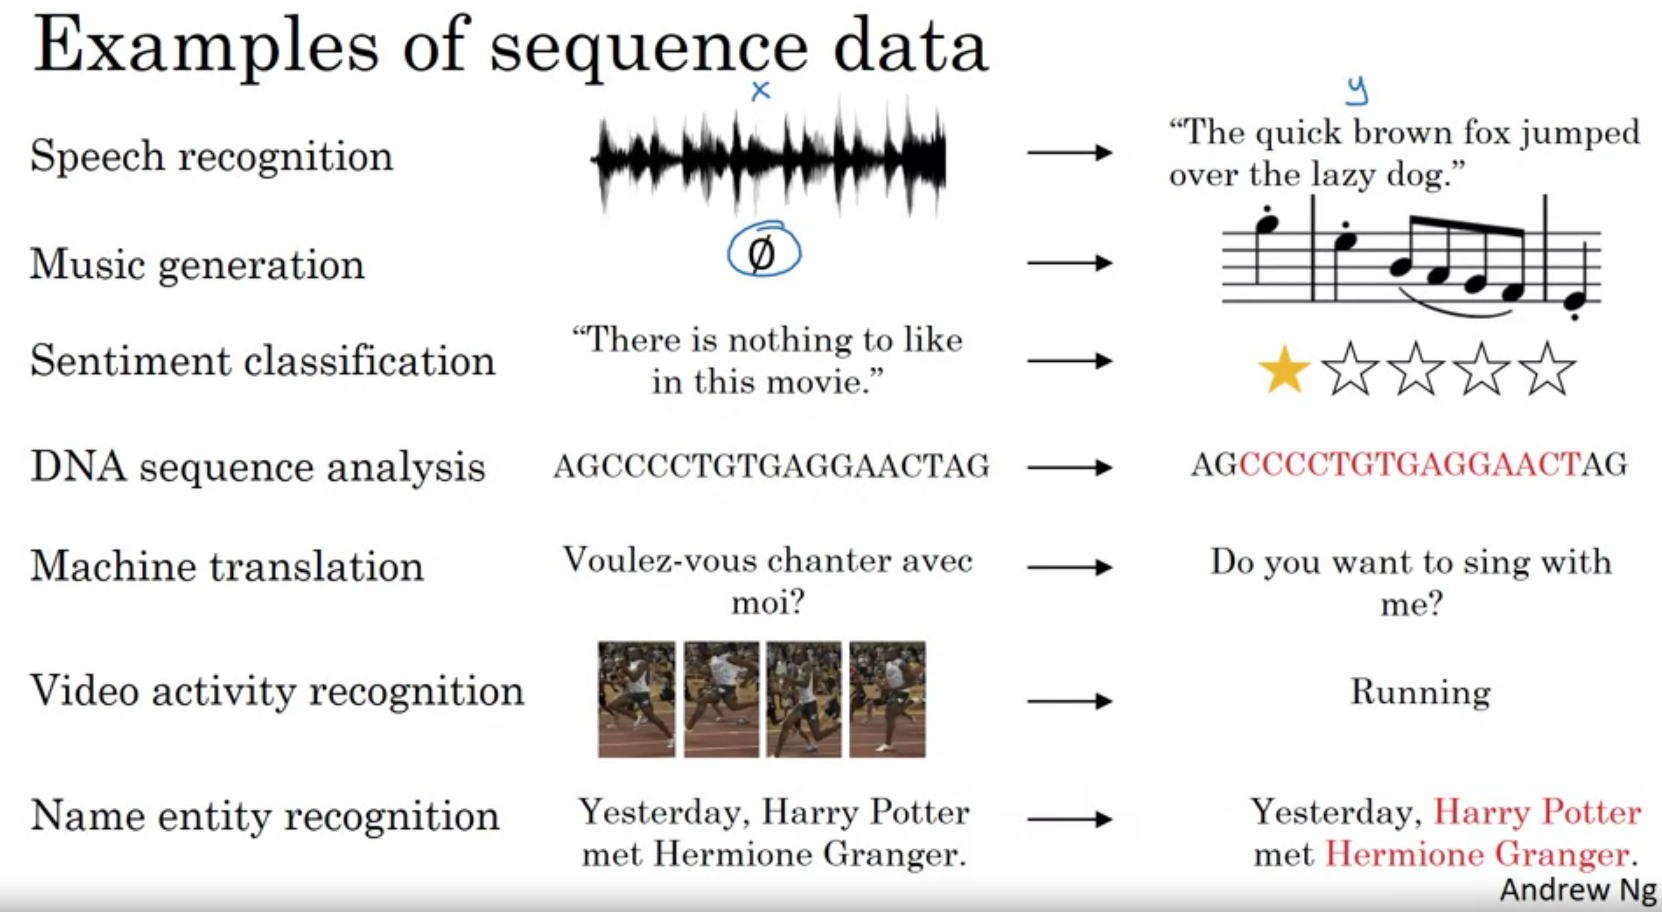
\includegraphics[width=12cm, height=8cm]{images/rnn_applications.png}    
    \end{center}
\end{frame}



\begin{frame}{Why not a Feed-forward Neural Network?}
    \begin{center}
        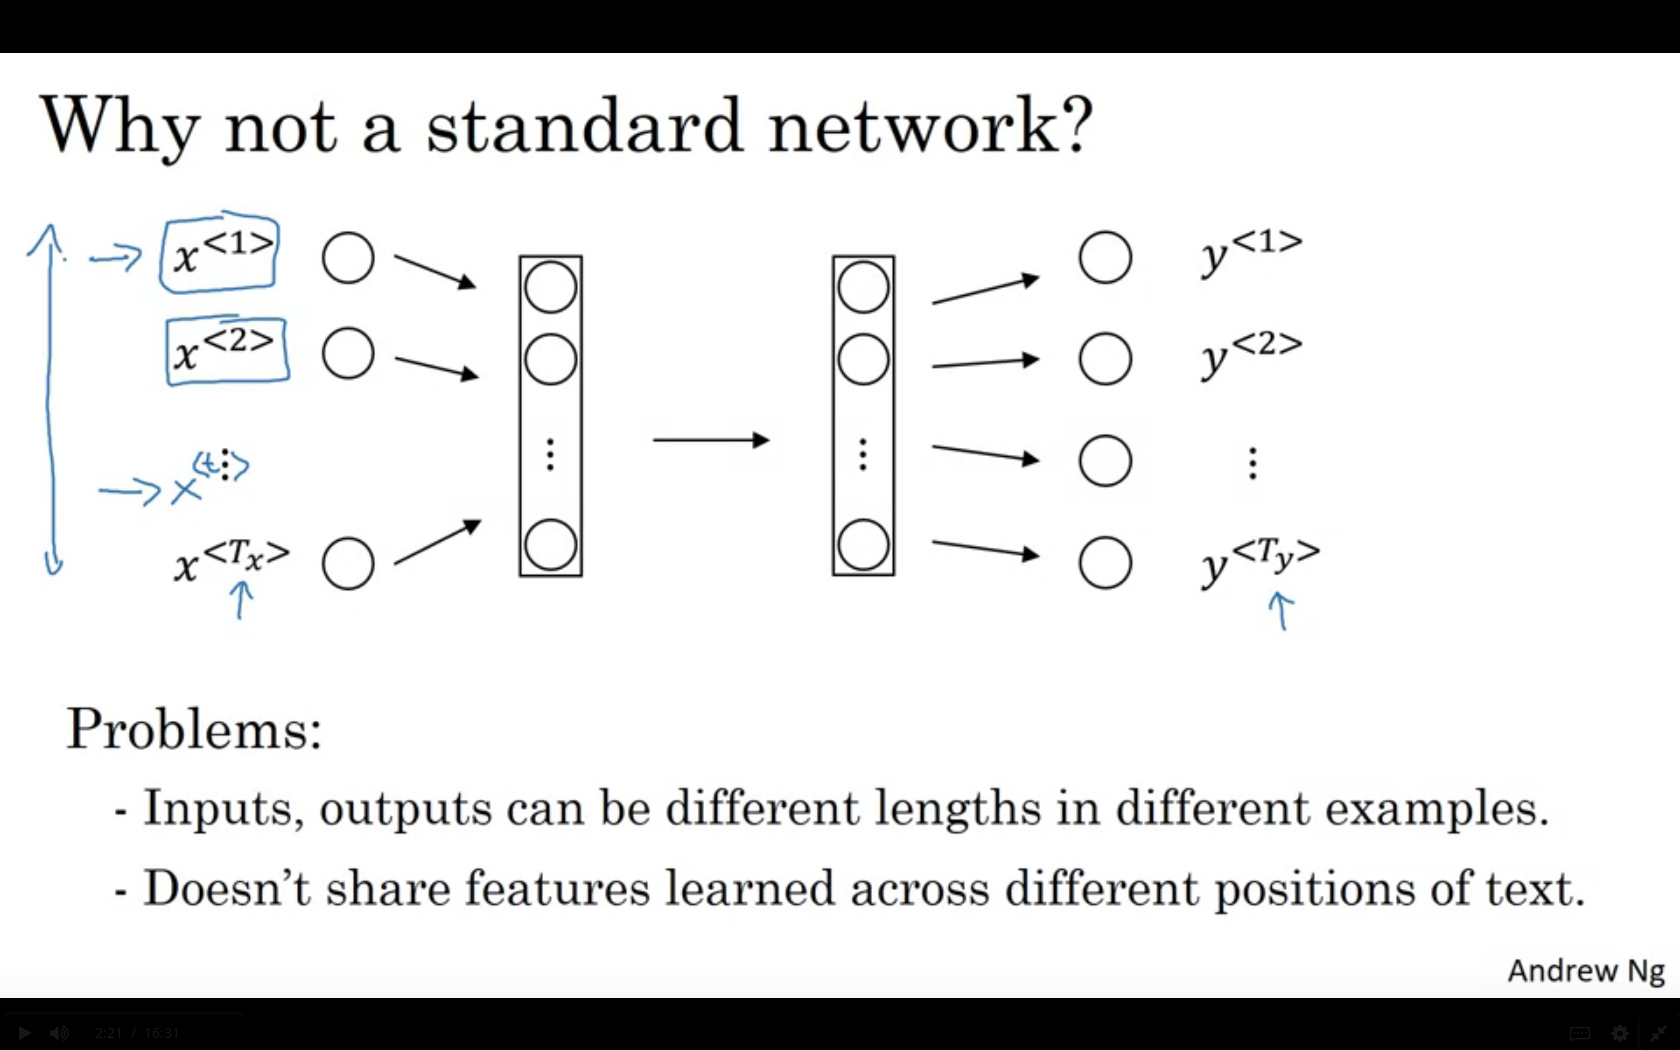
\includegraphics[width=12cm, height=8cm]{images/cnn_vs_rnn.png}    
    \end{center}
\end{frame}


\begin{frame}{RNN Cell}
    \begin{center}
        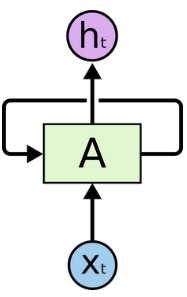
\includegraphics[width=3cm, height=4cm]{images/rnn_colah_blog.png}    
    \end{center}
\end{frame}

\begin{frame}{Unrolling}
    \begin{center}
        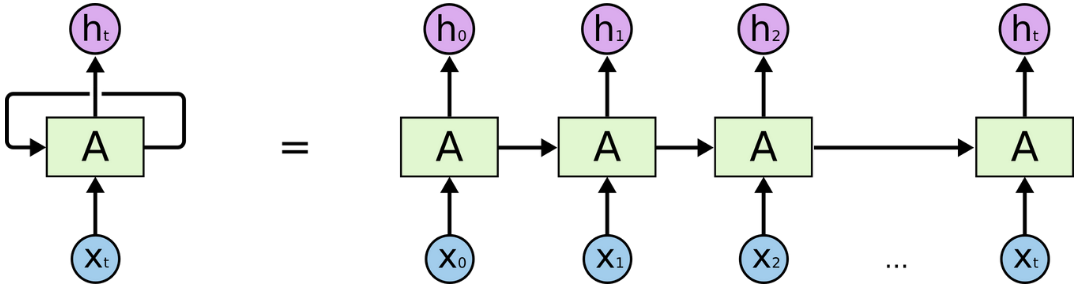
\includegraphics[width=10cm, height=4cm]{images/rnn_unrolled_colah_blog.png}    
    \end{center}
\end{frame}

\begin{frame}{Short-term dependencies: No issues}
    \begin{center}
                 \begin{figure}
            \centering
             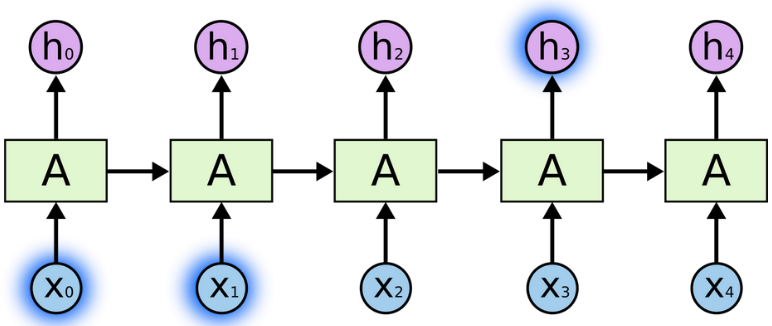
\includegraphics[width=10cm, height=4cm]{images/rnn_long_range_prob_1_colah.png}
            \caption{ Consider text auto-completion: \textit{The boy liked \big<NEXT WORD?? his/her/etc \big> bicycle...}}
            
        \end{figure}  
    \end{center}
\end{frame}

\begin{frame}{Long-term dependencies: Vanishing(or Exploding) Gradients}
    \begin{center}
        \begin{figure}
            \centering
            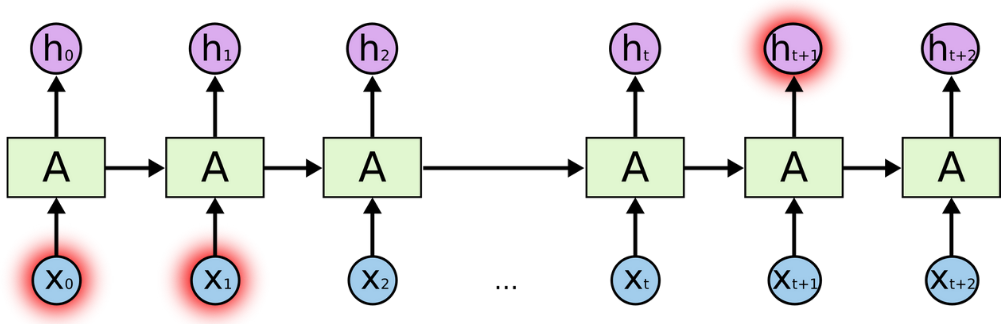
\includegraphics[width=10cm,height=4cm]{images/rnn_long_range_prob_2_colah.png}
            \caption{ Consider: \textit{A BARC employee, working on ...., published \big<NEXT WORD, \textit{(his or their??)}\big>...}. \textbf{Solution:} Need to cherrypick info.}
            \label{fig:my_label}
        \end{figure}
        
        
    \end{center}
\end{frame}

\begin{frame}{Inside a RNN cell}
    \begin{center}
        \begin{figure}
            \centering
                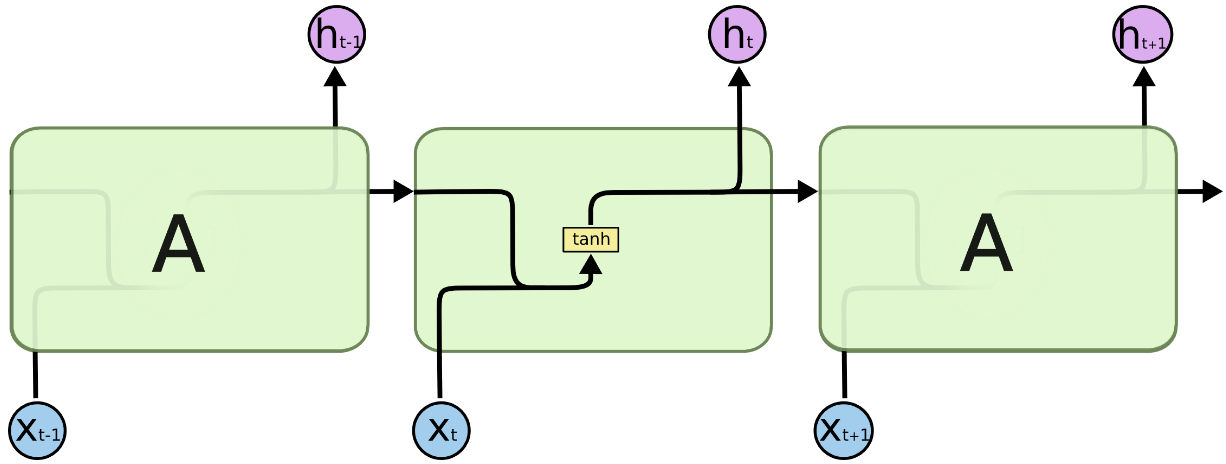
\includegraphics[width=10cm, height=4cm]{images/rnn_layer_colah.png} 
                \caption{No mechanism to cherry-pick,  \textit{\textbf{A BARC employee, working on ...., published} \big<NEXT WORD, \textit{(his or their??)}\big> ...}.}
        \end{figure}
        
    \end{center}
\end{frame}

\begin{frame}{LSTM cell}
    \begin{center}
        \begin{figure}
            \centering
                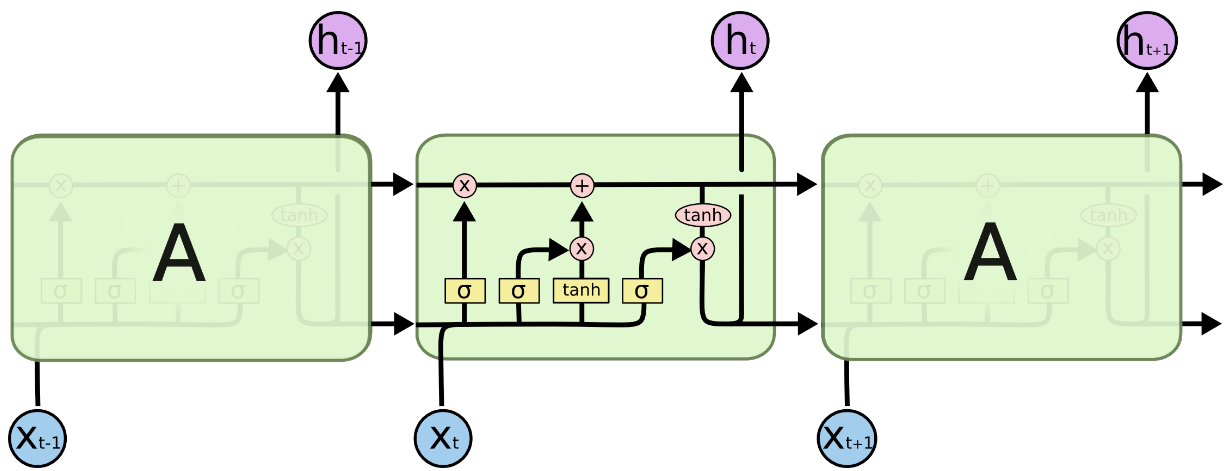
\includegraphics[width=10cm, height=4cm]{images/lstm_layer_colah.png}    
                \caption{Gating mechanism for cherry-picking,  \textit{\textbf{A} BARC employee, working on ...., published \big<NEXT WORD, \textit{(his or their??)}\big>...}.}
        \end{figure}
    \end{center}
    
\end{frame}

\begin{frame}{Cell state}
    \begin{center}
       \begin{figure}
           \centering
            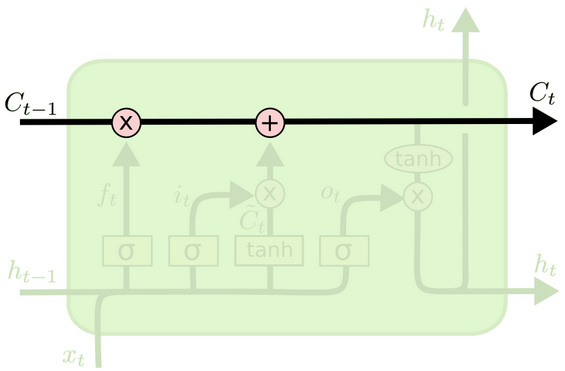
\includegraphics[width=6cm, height=4cm]{images/lstm_carry_over_colah.png}    
        \caption{Stores relevant context,  \textit{\textbf{A} BARC employee, working on ...., published \big<NEXT WORD\big> ...}, \textbf{A} implies Singular.}
        \end{figure}
    \end{center}
\end{frame}

\begin{frame}{LSTM Gate}
    \begin{center}
        \begin{figure}
            \centering
                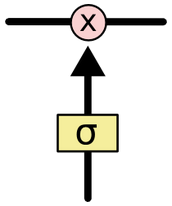
\includegraphics[width=3cm, height=4cm]{images/lstm_gate_colah.png}    
                \caption{Controls the relevance of last state, input and candidate output in determining the final state and output of a LSTM cell}
        \end{figure}       
    \end{center}
\end{frame}

\begin{frame}{LSTM Walkthrough: Forget control signal}
    \begin{center}
       \begin{figure}
           \centering
                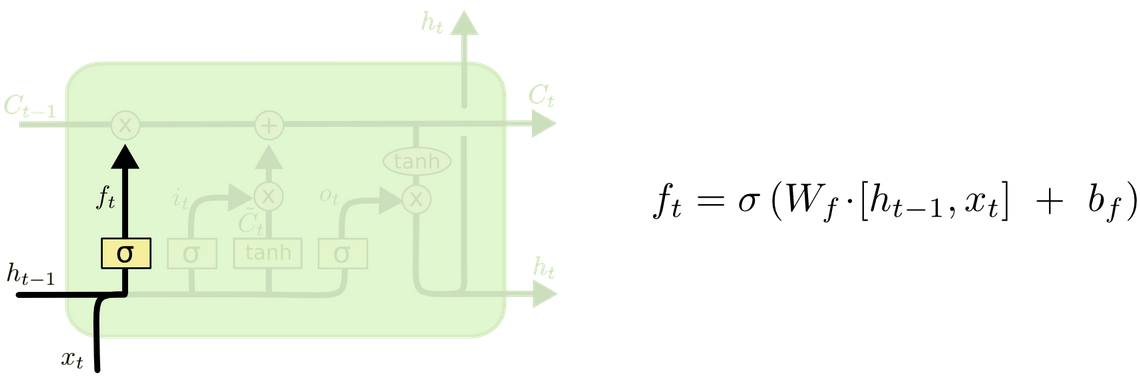
\includegraphics[width=10cm, height=4cm]{images/lstm_cell_ft_colah.png}
                \caption{Controls relevance of the state of previous cell for the current cell, \textit{\textbf{A} BARC employee, working on ...., published \big<NEXT WORD, \textit{(his or their??)}\big> ...}, focus on state of cell representing \textbf{A} only and reject state updates from other cells.}
        \end{figure}   
    \end{center}
\end{frame}

\begin{frame}{LSTM Walkthrough: Input control signal}
    \begin{center}
       \begin{figure}
           \centering
                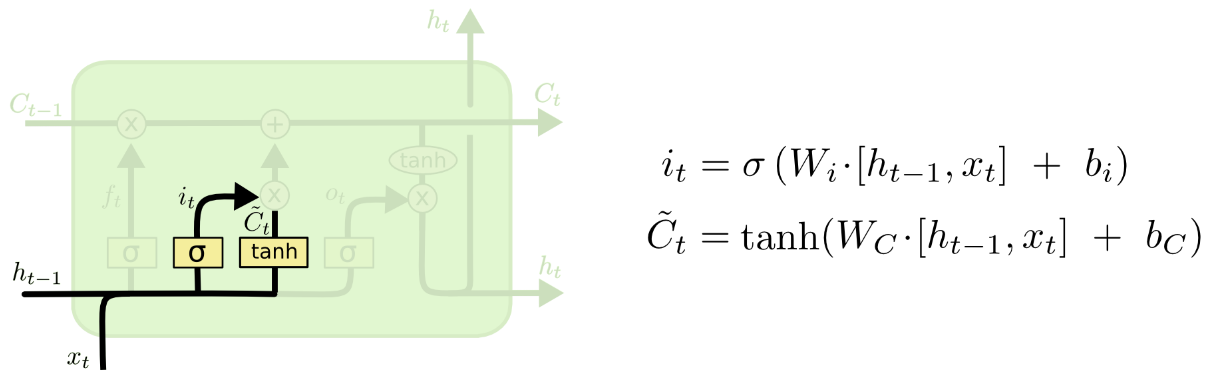
\includegraphics[width=10cm, height=4cm]{images/lstm_cell_c_t_colah.png}
                \caption{Controls relevance of the input for the current cell, \textit{\textbf{A} BARC employee, working on ...., published \big<NEXT WORD, \textit{(his or their??)}\big> ...}, words other than \textbf{A} will not be allowed to alter the state of their cells}
        \end{figure} 
        
        
        
        
    \end{center}
\end{frame}

\begin{frame}{LSTM Walkthrough: Forget and Input gate}
    \begin{center}
        \begin{figure}
            \centering
                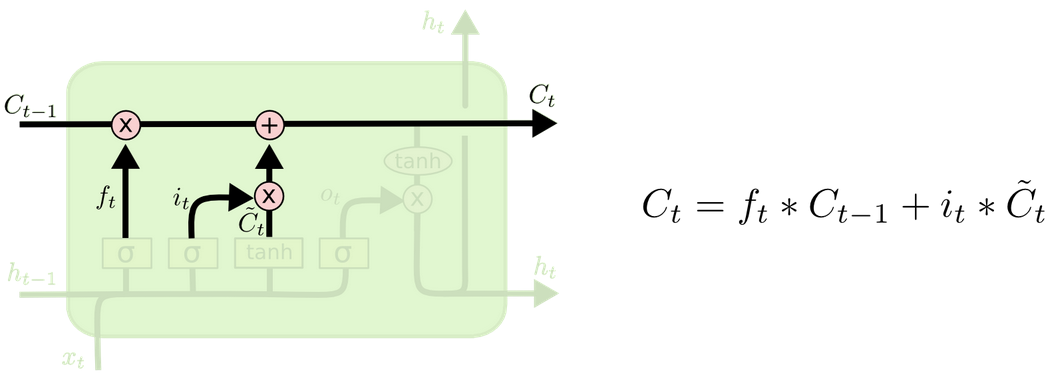
\includegraphics[width=10cm, height=4cm]{images/lstm_cell_C_t_colah.png}
                \caption{Cells state is an additive combination of input and last state controlled by respective gates. For above application, any cell between \textbf{A} and \big<WORD PREDICTION\big> cell will have \textit{singular} as the state update and no contributions from their word input.}
        \end{figure}
        
    \end{center}
\end{frame}

\begin{frame}{LSTM Walkthrough: Output gate}
    \begin{center}
        \begin{figure}
            \centering
                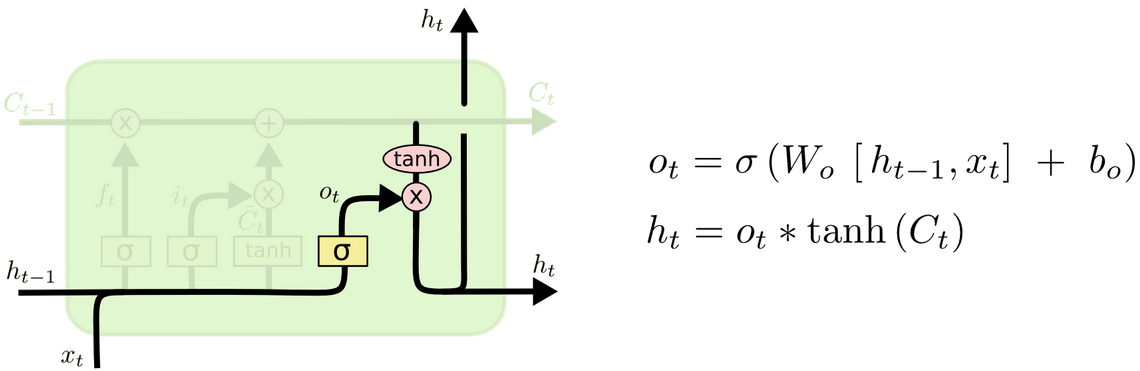
\includegraphics[width=10cm, height=4cm]{images/lstm_cell_h_t_colah.png}   
                \caption{Controls the relevance of current cell output depending on target application.In our auto-completion application, next word prediction is generated via output gate from one cell only, output signal from rest of the cells stays shut via output gate.}
        \end{figure}        
    \end{center}
\end{frame}


\begin{frame}{References}
    \begin{itemize}
        \item http://colah.github.io/posts/2015-08-Understanding-LSTMs/
        \item https://www.coursera.org/learn/nlp-sequence-models
        \item https://arxiv.org/abs/1507.05717
        \item https://distill.pub/2019/memorization-in-rnns/
    \end{itemize}
\end{frame}

\begin{frame}{}

    \begin{center}
        Thank you!!
    \end{center}
    
\end{frame}




%----------------------------------------------------------------------------------------
%	PRESENTATION SLIDES
%----------------------------------------------------------------------------------------

%------------------------------------------------

\end{document}

